\subsection{Décimo \textit{sprint} de producción}
El objetivo del décimo sprint es integrar los actores y controladores del juego 
para la creación de niveles completos y funcionales. De igual forma se 
implementa la funcionalidad faltante del menú principal y se construye el menú 
de selección de nivel.
\\
\par
Al cierre del octavo \textit{sprint} se generó una escena base para construir el 
resto de los niveles faltantes; por lo que en las siguientes secciones de este 
\textit{sprint} se abordan los pasos generales para la construcción de un nivel 
en su totalidad. Estos pasos se repiten para la creación de los niveles pero por 
la extensión del documento y para facilitar la lectura solo se hablan de los 
pasos para un solo nivel pero es importante que se considere que fue más de un 
nivel el que se construyó en este \textit{sprint}. 
\subsubsection{Construcción del escenario}  
Lo primero que se hace durante la creación de un escenario es la creación del 
suelo. En los primeros prototipos se emplearon dos métodos diferentes para esta 
tarea:  
	\begin{itemize}
		\item \textbf{\textit{Lever Builder}}: esta herramienta permite maquetar 
		niveles. Cuenta con tres modos: 
		\begin{itemize}
			\item \textbf{} Este modo sustituye el icon\textit{Print Mode:}o del 
			cursor por una mano y un cuadrado. Este permite agregar 
			\textit{sprites} oprimiendo el botón derecho y arrastrando el cursor 
			como si se tratara de un pincel. Para poder agregar \textit{sprites} 
			es necesario agregarlos anteriormente como componentes, ver figura 
			\ref{fig:LevelBuilder}.
			\item \textbf{\textit{Collider Mode:}}Utilizando el cursor de 
			cuadro, se seleccionan los componentes a los que se desea agregar un 
			colisonador. En este modo también se puede configurar el tipo de 
			colisionador que se desea agregar y la orientación del mismo 
			(vertical u horizontal), ver figura \ref{fig:LevelBuilder02}.
			\item \textbf{\textit{Selection Mode:}} \textit{Level Builder} 
			gestiona los \textit{sprites} a partir de generar parentescos con 
			objetos base que agrupan los \textit{sprites}; por ejemplo, los 
			\textit{sprites} referentes al suelo son hijos de un 
			\textit{GameObject} llamado \textit{Ground}. En este modo se puede 
			cambiar el objeto padre de los componentes seleccionados, 
			duplicarlos, encontrarlos en la pestaña de jerarquía, etc.  
		\end{itemize} 
		
		El principal problema que se tuvo con esta herramienta fue que no 
		agilizaba el maquetado de los niveles significativamente, llegando 
		incluso a complicar más la creación del suelo si por algún motivo se 
		debía de modificar el parentesco entre los componentes del suelo. Otro 
		inconveniente que presentaba esta herramienta es que requería de 
		configuraciones extras para generar la \textit{APK} del juego.
		
		\item \textbf{Acomodo manual de los \textit{Sprites:}} Esto consistía en 
		acomodar los \textit{sprites} de manera manual los \textit{sprites} 
		dentro de una escena. Esto no solo era tardado y laborioso sino que 
		también no proporcionaba una maquetación tan exacta ya que en teléfonos 
		de alta resolución se podían apreciar espacios entre los 
		\textit{sprites} que componen el suelo.
	\end{itemize}

La alternativa que se utiliza para estos dos métodos en la creación del 
escenario es utilizar un nuevo tipo de \textit{GameObject} llamado: 
\textit{\textbf{Tilemap}}. Este objeto crea una grilla virtual sobre la que se arrastraran los \textit{sprites} que se deseen agregar. El tamaño de los cuadros que componen la grilla puede ser configurado modificando los valores del atributo \textit{Tile Anchor}, para este proyecto el valor para \textit{X} y \textit{Y} es de $0.5$. Para poder agregar \textit{sprites} a la grilla es necesario crear primero un \textit{Tile Palette}. Para crear un \textit{Tile Palette} se dirige el cursor a la pestaña de \textit{Tile Palette} y se da click en la opción de \textit{Create new palette}, ver figura . una vez hecho esto se va a abrir un cuadro de dialogo en donde se le asigna un nombre al \textit{palette} creado, para este proyecto el \textit{palette} tiene por nombre \textit{Ground}, ver figura . Elegido el nombre, se da click en el botón de \textit{create} y se abre una nueva pestaña en la que se debe seleccionar la locación donde se va a guardar el \textit{palette}, en este caso se elige una carpeta llamada \textit{Tiles}. Como paso final se deben de agregar \textit{sprites} al \textit{palette}, esto se logra arrastrando los sprites que se desean agragar a la grilla de la pestaña \textit{Tile Pilette}, ver figura. Con estos pasos completados se procede a pintar el nivel. \textit{Unity} ofrece diferentes herramientas para rellenar la grilla, tales como: el pincel que permite poner un \textit{sprite} cuadro por cuadro; \textit{Filled Box} que permite rellenar áreas enteras; el borrador, que permite eliminar \textit{sprites}, etc. En la figura se muestra el uso de la herramienta \textit{Filled Box} para dibujar una zona del suelo del nivel. Tomando la maqueta del nivel como base, se pinta todo el suelo. 
\\
\par
Es posible asignar un colisionador como componente a un \textit{GameObject} de 
tipo \textit{Tilemap}. Primeramente se agrega el componente \textit{Rigidbody 
2D} y se configura como del tipo \textit{Kinematic}. Luego se agrega el 
componente \textit{Composite Collider 2D}. Finalmente se agrega el componente 
\textit{Tilemap Collider 2D}, en este componente se activa la casilla de 
\textit{Used By Composite}. Con esta configuración \textit{Unity} genera los 
colisionadores de manera automática según las superficies utilizadas por los 
\textit{sprites} que hayan sido puestos en la grilla de la escena; lo anterior 
permite que el colisionador se actualice y adapte según se vayan agregando o 
quitando elementos a la grilla. En la figura se puede observar el colisonador de 
un nivel generado con estos componentes.
\\
\par
Terminado el suelo del nivel, se agregan los actores del nivel, es decir los enemigos, puntos de guardado, obstáculos, ítems y objetos coleccionables, en caso de que el tenga. Todos estos componentes únicamente se arrastran a la escena ya que en los \textit{sprints} anteriores fueron configurados para ser \textit{assets}. Una vez agregados a la escena, lo que queda es configurar el tamaño del area activa para las plataformas de algunos objetos, la cantidad de daño que los enemigos y algunos objetos pueden infringir y la cantidad de vida y \textit{tonalli} que los ítems pueden restaurar. 
\\
\par
Finalmente se agregan alguno sprites que corresponden a objetos de fondo. Por ejemplo en el nivel cuatro en la zona de plataformas hay antorchas que son objetos meramente decorativos, ver figura .

\begin{figure}[h]
		\centering
		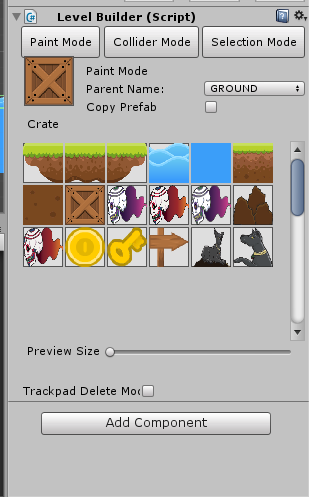
\includegraphics[height=0.2 \textheight]{03TrabajoRealizado/imagenes/levelBuilder02.png}
		\caption{Pestaña del \textit{Print Mode} de la herramienta \textit{Level 
		Builder.}}
		\label{fig:LevelBuilder}
\end{figure}

\begin{figure}[h]
		\centering
		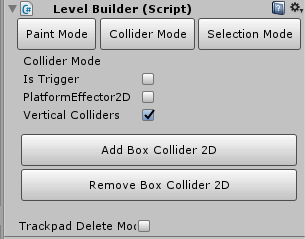
\includegraphics[height=0.2 \textheight]{03TrabajoRealizado/imagenes/levelBuilder03.png}
		\caption{Pestaña del \textit{Collider Mode} de la herramienta 
		\textit{Level 
		Builder.}}
		\label{fig:LevelBuilder02}
\end{figure}

\begin{figure}[h]
		\centering
		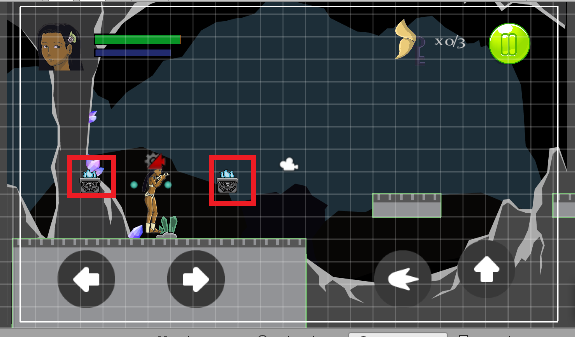
\includegraphics[height=0.2 \textheight]{03TrabajoRealizado/imagenes/objetosFondo.png}
		\caption{Encerradas por recuadros rojos se pueden ver las antorchas que decoran el nivel cuatro en la zona de plataforma.}
		\label{fig:ObjetoFon}
\end{figure}

\subsubsection{Configuración de la cámara}
Para lograr que la cámara siga al jugador se utiliza un \textit{asset} llamado 
\textit{Cinemachine}. En los prototipos anteriores se había empleado una clase 
llamada \textit{CameraCrl}, esta clase permitía que la cámara siguiera al 
jugador pero no lograba marcar limites para el movimiento de la cámara, lo que 
provocaba que la cámara mostrara espacios vacíos. \textit{Cinemachine} permite 
solucionar ese problema de una manera bastante sencilla pero primeramente se va 
a iniciar por hablar sobre su integración en el proyecto.
\\
\par
\textit{Cinemachine} es una herramienta desarrollada por \textit{Unity}; no obstante, no viene por defecto con la versión 2017 del software y es necesario descargarla desde la tienda de \textit{assets}, ver figura . Una vez que se descarga se debe de desempaquetar, ver figura . Para verificar que se ha integrado esta herramienta al proyecto en la barra de tareas principal debe de aparecer la opción \textit{Cinemachine}, ver figura ; de igual forma en las carpetas del proyecto debe de mostrarse una carpeta con el mismo nombre, ver figura. 
\\
\par
Para crear una cámara con \textit{cinemachine}, se debe dar click en la opción de \textit{cinemachine} de la barra principal de tareas y seleccionar la opción de \textit{Create 2D camera}, ver figura \ref{fig:CinemachineCreate}. Lo anterior va a crear una cámara virtual en la pestaña de jerarquía, ver figura . Para vincular la cámara virtual con la cámara principal se debe de agregar el componente de \textit{Cinemachine Brain} a la cámara principal. Lo que resta es configurar la cámara virtual para que siga al jugador. Se arrastra el \textit{GameObject} del jugador de la pestaña de jerarquía al atributo de \textit{Follow} de la cámara virtual; esto le indica a la cámara cual va a ser el objeto de debe de seguir. Al seleccionar la cámara virtual, se puede observar en la vista de \textit{Game} que la pantalla tiene dos zonas una azul y otra roja; la zona azul delimita el área en la que el jugador puede moverse sin que la cámara lo siga y una vez que se aproxima a la zona roja, la cámara comienza a seguirlo, ver figura \ref{fig:CameraZones}. El tamaño de estas zonas puede ser modificado con los valores de los atributos \textit{Screen X, Screen Y, Dead Zone Width} y \textit{Dead Zone Heidth}, ver figura \ref{fig:CameraAttibutes}. 
\\
\par
Para finalizar la configuración de la cámara se crea el área que contendrá la cámara, es decir el área de la que la cámara no puede salir. Para tener un area de contención, primero se debe de crear un \textit{GameObject} vació nuevo, para este proyecto este \textit{GameObject} se llama \textit{LimitCamera}. A \textit{LimitCamera} se le agrega el componente \textit{Polygon Collider}, se configura el colisionador como de tipo \textit{Trigger} y se modifica su forma para que se adapte al mapeado del nivel, en la figura se muestra un ejemplo de la forma que se le dio a este \textit{GameObject}. Finalmente se agrega el componente \textit{Cinemachine Confiner} a la cámara virtual y se arrastra a \textit{LimitCamera} al atributo \textit{Bounding Shape 2D}, ver figura \ref{fig:CameraLimit}. Con esto se logra que los limites de \textit{LimitCamera} sean los limites de la cámara.

\begin{figure}[h]
		\centering
		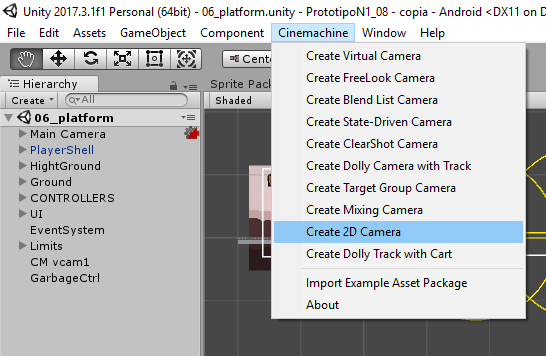
\includegraphics[height=0.2 \textheight]{03TrabajoRealizado/imagenes/cinemachine0001.png}
		\caption{Creación de una camara de tipo \textit{cinemachine}.}
		\label{fig:CinemachineCreate}
\end{figure}

\begin{figure}[h]
		\centering
		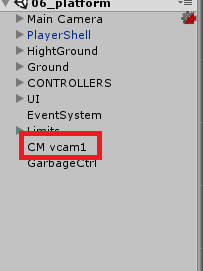
\includegraphics[height=0.2 \textheight]{03TrabajoRealizado/imagenes/cinemachine0002.png}
		\caption{Cámara virtual desde la pestaña de jerarquía.}
		\label{fig:VitualCamera}
\end{figure}

\begin{figure}[h]
		\centering
		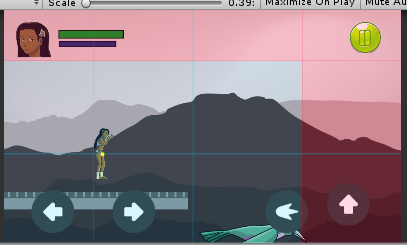
\includegraphics[height=0.2 \textheight]{03TrabajoRealizado/imagenes/cinemachine0003.png}
		\caption{La zona azul corresponde al área que en la que el jugador puede moverse dentro del juego sin que la cámara lo siga.}
		\label{fig:CameraZones}
\end{figure}

\begin{figure}[h]
		\centering
		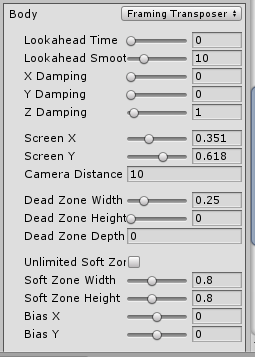
\includegraphics[height=0.2 \textheight]{03TrabajoRealizado/imagenes/cinemachine0004.png}
		\caption{Atributos que se pueden modificar para cambiar las dimensiones de la zona azul de la cámara virtual.}
		\label{fig:CameraAttibutes}
\end{figure}

\begin{figure}[h]
		\centering
		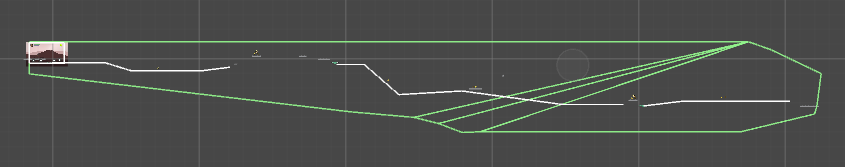
\includegraphics[height=0.1 \textheight]{03TrabajoRealizado/imagenes/cinemachine0005.png}
		\caption{Configuración de la forma de \textit{LimitCamera}.}
		\label{fig:CameraLimit}
\end{figure}


\subsubsection{Creando el controlador del nivel}
El controlador del nivel es aquel que se encarga de verificar que el jugador 
haya cumplido con el objetivo del nivel y en caso de que lo haya cumplido el 
controlador debe de desbloquear el nivel siguiente y guardar el progreso del 
jugador. En total existen cuatro tipos de controladores de nivel:
\begin{itemize}
	\item El controlador que solo verifica que el jugador haya llegado al final 
	del nivel.
	\item El controlador que verifica que el jugador haya llegado al final del 
	nivel y haya recolectado una cantidad determinada de objetos colleccionables 
	pero no guarda el marcador.
	\item El controlador que verifica que el jugador haya llegado al final del 
	nivel y guarda el valor del marcador.
	\item El controlador que verifica que el enemigo de tipo jefe haya sido 
	eliminado.
\end{itemize} 

El primer tipo de controlador es empleado en la zona de plataforma de los 
niveles seis y ocho. El segundo se emplea en la zona de plataforma del nivel 
cuatro. El tercer tipo se emplea en la zona de plataforma del segundo nivel. 
Mientras que el último controlador se utiliza para las zonas de jefe de todos 
los niveles.
\\
\par
En lo que se refiere a la progresión del personaje, es decir al aumento de la 
vida, cantidad de \textit{tonalli} y cantidad de daño de \textit{Malinalli}, en 
la figura se muestra la progresión del personaje una vez que el jugador ha 
terminado un nivel determinado.


\subsubsection{Creación de las cinemáticas del juego}
En este \textit{sprint} se crean las cinemáticas de los niveles pares. Las cinemáticas del juego son aquellas animaciones que fungen como transiciones entre escenas, su objetivo es el de contar la historia del juego.
\\
\par
Una escena de tipo cinemática tiene tiene la siguiente estructura visual(ver figura \ref{fig:Cinematica}):
	\begin{itemize}
		\item Una imagen que contiene  los diálogos.
		\item Un objeto de texto para el nombre del personaje.
		\item Un objeto de texto para el dialogo.
		\item Un objeto de texto para indicarle al jugador que debe de oprimir el botón de salto para ver el siguiente dialogo.
		\item Botones que controlan al jugador en los niveles.
		\item \textit{Sprites} de los personajes que aparecen en esa escena. 
	\end{itemize}
Para la creación de la cinemáticas se emplean los diálogos del guión literario desarrollado durante el trabajo termina 1 y las imagenes correspondientes al diseño de personajes también realizadas durante trabajo terminal 1. 
\\
\par
Las clases encargada del controlar el flujo de los diálogos en la cinemática son las clases \textit{DialogueCtrl} y \textit{DialogueFile}. Como se menciona en la sección \ref{ControladorDialogo}, estas clases se encargan de la visualización y transición de diálogos.

\begin{figure}[h]
		\centering
		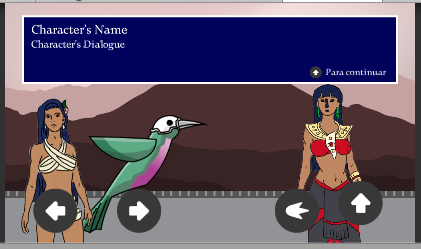
\includegraphics[height=0.3 \textheight]{03TrabajoRealizado/imagenes/cutscene.png}
		\caption{Estructura visual de una escena de tipo cinemática.}
		\label{fig:Cinematica}
\end{figure}

\subsubsection{Agregando la funcionalidad faltante al menú principal}
La funcionalidad faltante del menú principal es la verificación de la existencia del archivo que contiene los datos de la partida, en caso de que no exista el archivo crearlo, en caso de que exista cargar la información y la aparición de los mensajes de confirmación. En los primeros prototipos el menú principal dirigía al jugador y no permitía que el jugador guardará su progreso.
\\
\par
Para conseguir el funcionamiento ya descrito, se crea la clase \textit{MenuCrl} 
y se agrega un \textit{GameObject} de tipo \textit{Panel} como el que se ve en 
la figura \ref{fig:menuctrlPanel}, este panel tiene esa estructura a fin de ser 
utilizado tanto para el mensaje de advertencia para crear una nueva partida como 
para el mensaje que notifica que no existe una partida previamente guardada.
Cuando el jugador oprime el botón de \textit{Empezar partida}, se manda a llamar 
al método \textit{OpenWarnningWindow}, este método habilita el panel del mensaje 
y modifica el texto que se muestra en el panel por el: “Advertencia: Se 
eliminarán todos los datos previamente guardados. ¿Desea crear una nueva 
partida?". Si el jugador oprime el botón de aceptar el \textit{MenuCtrl} mandará 
a llamar el método \textit{CreateNewGameData} de la clase \textit{GameDataCtrl} 
y cargara la escena del menú de selección de partida. Si el jugador oprime el 
botón de cancelar, el \textit{panel} de advertencia se cerrará. En caso de que 
el jugador quiera cargar su partida, éste debe de oprimir el botón de 
\textit{Cargar partida}, lo que manda a llamar el método \textit{LoadGame} de la 
clase \textit{MenuCtrl}; el método \textit{LoadGame} verifica si existe el 
archivo con los datos de la partida, su existe se cargan los datos y se redirige 
a la pantalla de selección de nivel, en caso contrario se habilita el 
\textit{panel} con el aviso de que no se encontró ningún archivo con los datos 
del juego y se le pide al jugador iniciar una nueva partida. 

\begin{figure}[h]
		\centering
		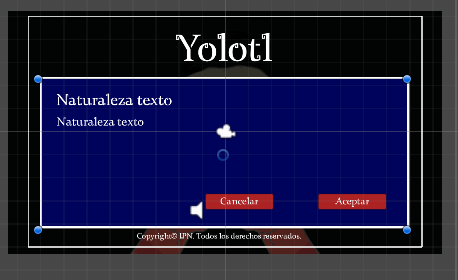
\includegraphics[height=0.2 \textheight]{03TrabajoRealizado/imagenes/menuctrlPanel.png}
		\caption{\textit{Panel} agregado a la interfaz del menú principal a fin 
		de mostrar los mensajes de confirmación de crear nueva partida o para 
		notificar que no existe una partida previamente guardada.}
		\label{fig:menuctrlPanel}
\end{figure}
 
\subsubsection{Creación de la funcionalidad del menú de selección de nivel}
El menú de selección de nivel, es el encargado de permitirle al jugador seleccionar que nivel desea jugar. El jugador solamente puede acceder a los niveles que haya desbloqueado. 
\\
\par
Para implementar este menú se crea primeramente la intefaz grafica. Esta se logra con tes botones (dos para navegar y uno para confirmar que nivel se desea seleccionar), tres imágenes (Dos para el cuadro de texto donde se muestra la información del nivel y una para la imagen del nivel) y dos objetos de texto (para el titulo del nivel y la descripción del nivel). En la figura \ref{fig:menuSelectIntefaz} se muestra la interfaz del menú de selección de nivel. 
\\
\par
Para dar la impresión al jugador de que se encuentra ante una navegación de tipo carrusel, la clase \textit{SelectionManuCtrl}(encargada de la funcionalidad del menú de selección de nivel) se vale de recorrer tres arreglos para modificar el contenido de la interfaz. Los tres arreglos son los siguientes:
\begin{itemize}
	\item \textit{\textbf{LevelInformation}}: Arreglo de instancias de la clase auxiliar \textit{LevelDescriptor}, \textit{LevelDescriptor} tiene como atributos dos \textit{strings} correspondientes al nombre del nivel y a la descripción del nivel.
	\item \textit{\textbf{levelImage}}: Arreglo de \textit{sprites}, los \textit{sprites} de este arreglo corresponden a las imagenes de los niveles.
	\item \textit{\textbf{levelName}}:	Este arreglo de \textit{strings} corresponde al nombre de las escenas de los niveles para ser cargadas.	
\end{itemize}  
\textit{SelectionManuCtrl} se vale de dos métodos: \textit{GoNext} y \textit{GoPrevious} para navegar a través de los arreglos y mostrar la información de los niveles si estos ha sido desbloqueados por el jugador, de lo contrario muestran por defecto el mensaje de “No disponible”, ver figura  \ref{fig:MenuSelect}.   

\begin{figure}[h]
		\centering
		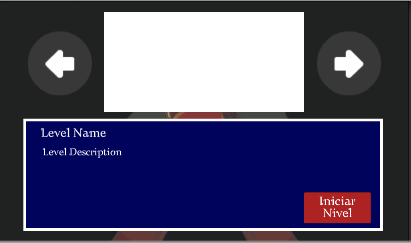
\includegraphics[height=0.2 \textheight]{03TrabajoRealizado/imagenes/menuctrlPanel04.png}
		\caption{Diseño del menú de selección de nivel}
		\label{fig:menuSelectIntefaz}
\end{figure}


\begin{figure}
  \centering
   \subfigure[Vista del menú de selección de nivel cuando el nivel no ha sido desbloqueado] {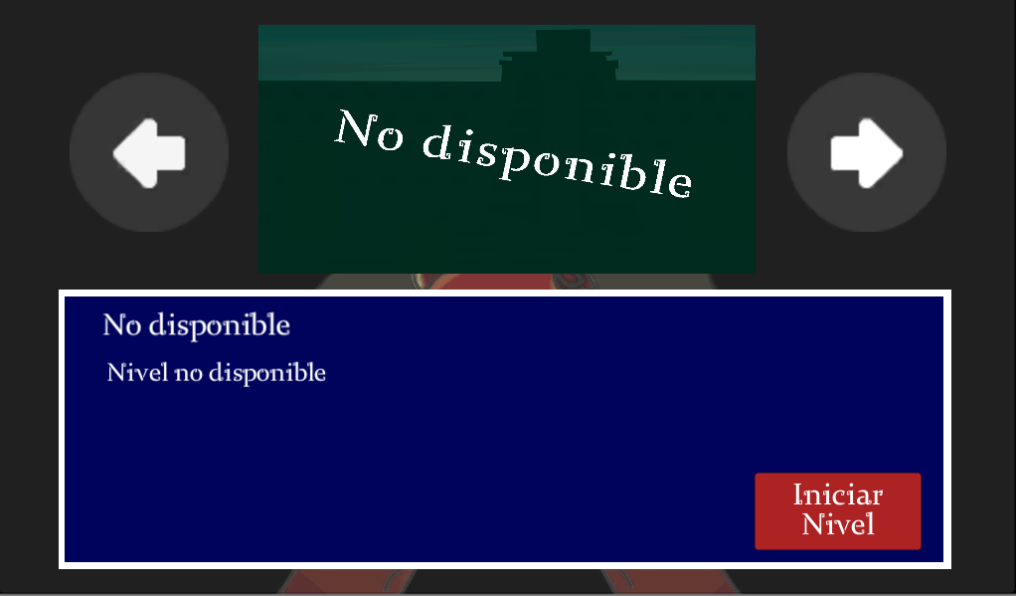
\includegraphics[width=0.5 \textwidth]{03TrabajoRealizado/imagenes/menuctrlPanel02}}
   
 	\subfigure[Vista del menú de selección de nivel cuando el nivel ha sido desbloqueado.] {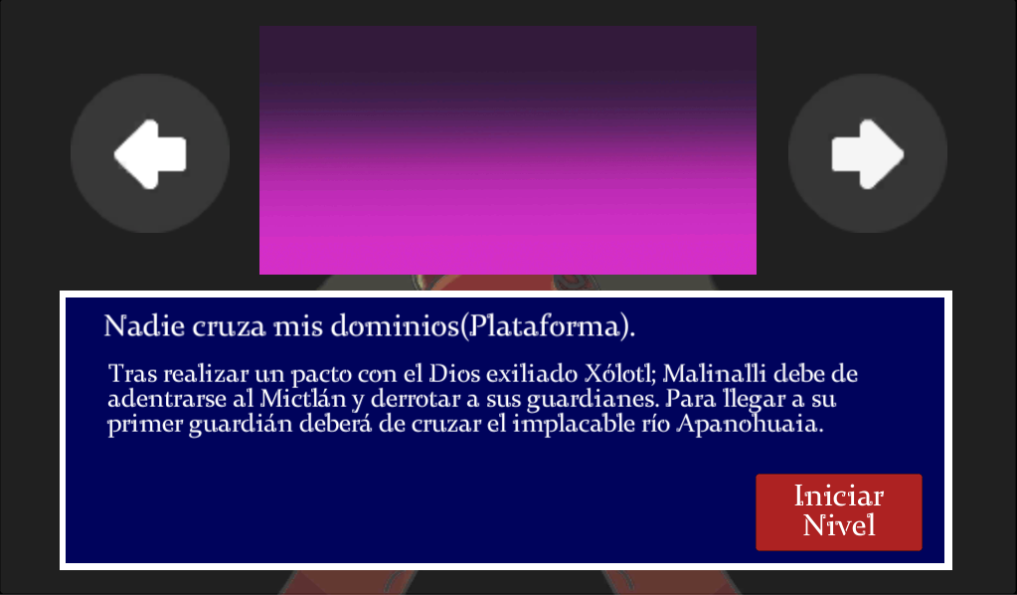
\includegraphics[width=0.5 \textwidth]{03TrabajoRealizado/imagenes/menuctrlPanel03}}
 	
  \caption{Vistas del menú de selección de nivel dependiendo de si el nivel esta o no disponible.}
  \label{fig:MenuSelect}
\end{figure} 

\subsubsection{Cierre del sprint}
Al cierre de este \textit{sprint} se cuenta con los niveles terminado y funcionales 
así como los menús del juego. Por lo que se deja todo preparado para la realización 
de pruebas.